\chapter{Design}
\label{ch:design}
In this chapter we will discuss the architecture of the prototype.
It's divided into two sections: Dataset and Model. Since
the dataset is standalone component, this seems to be
a reasonable separation. To make it clear, dataset would be a component
that holds the training, validation and test data including all relevant
functionality that can or should be performed on the
data(this is explained in more detail in \autoref{sec:design_data}).
The model is a component, which accepts the data(dataset component), performs
training on the training data, and then makes inference on the test dataset.
In other words, the model would be everything that is related to building,
training and the evaluation of neural networks and reinforcement learning environment.



\section{Dataset}
\label{sec:design_data}

The dataset is component that is responsible for data holding. It should
accept original MNIST dataset and transform it into dataset described
in \autoref{sec:analysis_dataset}.

% For example, in the figure \ref{fig:mnist} the labels are 5, 0, 4 and 1.
% Each images consist of $28\times28$ pixels, therefore an MNIST image would
% be an array of size $784$. To each of the image, a label is assigned,
% which provides the ground truth.

\subparagraph{MNIST dataset from TensorFlow}

TensorFlow provides a small class \lstinline{Dataset}\footnote{
The class is implemented here on tensorflow Github repository under the path: \lstinline{tensorflow/contrib/learn/python/learn/datasets/mnist.py}.
} which stores MNIST data and splits it into training,
validation and test data. TensorFlow also provides functions for iterating
over the batches as well as the function which downloads and read
the original data
from MNIST web site. Taking this into account, in this work we will abstract from
downloading and reading MNIST data by using this class. We'll refer
to this class as \emph{MNIST tf-dataset class}.

% Remove this:
% \begin{lstlisting}[language=Python]
% from tensorflow.examples.tutorials.mnist import input_data
% mnist = input_data.read_data_sets("MNIST_data/", one_hot=True)
% \end{lstlisting}
% This two lines will download the data and store into "MNIST_data/" directory.

We want that our dataset component has a similar behaviour and functionally
as MNIST tf-dataset class. The reason for this is that we want to stay
consistent with TensorFlow practices as we use this library in this work.

% Dataset is a non-real world data, but may behave and represent similar
% task as it could in real world data.
% \paragraph{explain original MNIST data, what is there, how does this work,
% and tf class is used to provide the utility}

% \paragraph{Obstacles} Using the procedure described in \autoref{sec:design_data}
% to create the dataset several obstacles can arise.
% we need to make sure that no same non-noise picture come up with in the dataset.

% To make the dataset
% By build the dataset, we need to consider following

% we want the model to generalise on unseen data.

\subsection{Architecture}

Before proceeding with the classes overview, it can be helpful
to make a concrete example of how the dataset described in
\autoref{sec:analysis_dataset} can look like.

\paragraph{Example} In this example we will describe dataset with two classes
Let's first choose the parameters $n$ and $k$,
which represents the number of images in a group and the amount of noise images
in a group respectively. While $k$
should be different for both classes, $n$ remains the same.
Let $n$ be equal to $5$, $k$ for the first class be and $3$: $k_1 = 3$
for the second class be $4$: $k_2 = 4$. Let's choose the digit for the non-noise
data: $\{1\}$. Consequentially the noise-image will
be: $\{0, 2, 3, 4, 5, 6, 7, 8, 9\}$.
So one sample of the above mentioned setup can look like this:

\begin{lstlisting}[language=Python][h!]
	[noise_image, non_noise_image, noise_image, non_noise_image, noise_image ] # class 1
	[non_noise_image, noise_image, noise_image, noise_image, noise_image ] # class 2
\end{lstlisting}

Or with numbers:
\begin{lstlisting}[language=Python][h!]
	[9, 1, 8, 1, 7 ] # class 1
	[1, 3, 6, 4, 3 ] # class 2
\end{lstlisting}



\paragraph{Class overview}

It was decided that in order to implement
the desired dataset, three classes are required:
\begin{itemize}
	\item IndexGenerator - the purpose of this class is to generate indexes for
		noise images. Imagine situation, where all of noise data is placed into
		the same indexes. Will this model learn this indexes and look only at
		them? Or will model ignore this stability? Because this question seems
		to be heuristic, this class will control the indexes where noise image
		will be located at. By instantiating this class, it's possible to have
		always the same indixes for the noise images, as well as control it by
		providing discrete distribution function, where this indexes should be sampled from.
	\item DummyDataset - The purpose of this class is to hold MNIST images
		and labels. Additionally, this class provides some auxiliary functionality
		like permutation of the data.
	\item GroupDataset - this is our desired dataset. It should be flexible
		enough to generate and hold the data for all classes. In terms of
		available methods, this class behaves the same way as MNIST tf-dataset class.
\end{itemize}

Dataset component should be flexible enough in order to be similar to real problems,
to be able to experiment with different amount of classes, and
different variations of noises classes. Since we have only a limited amount of MNIST data,
we need to also make sure that this data is properly used. GroupDataset takes
care of it by carefully choosing the data from original MNIST dataset and putting
them into the group to avoid if possible two same samples in the dataset by building
combinations of noise-data and non-noise data.

\subsection{UML class diagram}

In the figure \ref{fig:dataset_uml} you can see UML diagram of the dataset package
as well as the it's connection to tf-dataset class. As you can see from the UML
class diagram.
\lstinline{GroupDataset} class holds two \lstinline{DummyDataset}, one for
non-noise data and one for noise-data. This is exactly the way
we described it in \autoref{sec:analysis_dataset}.
\begin{figure}
	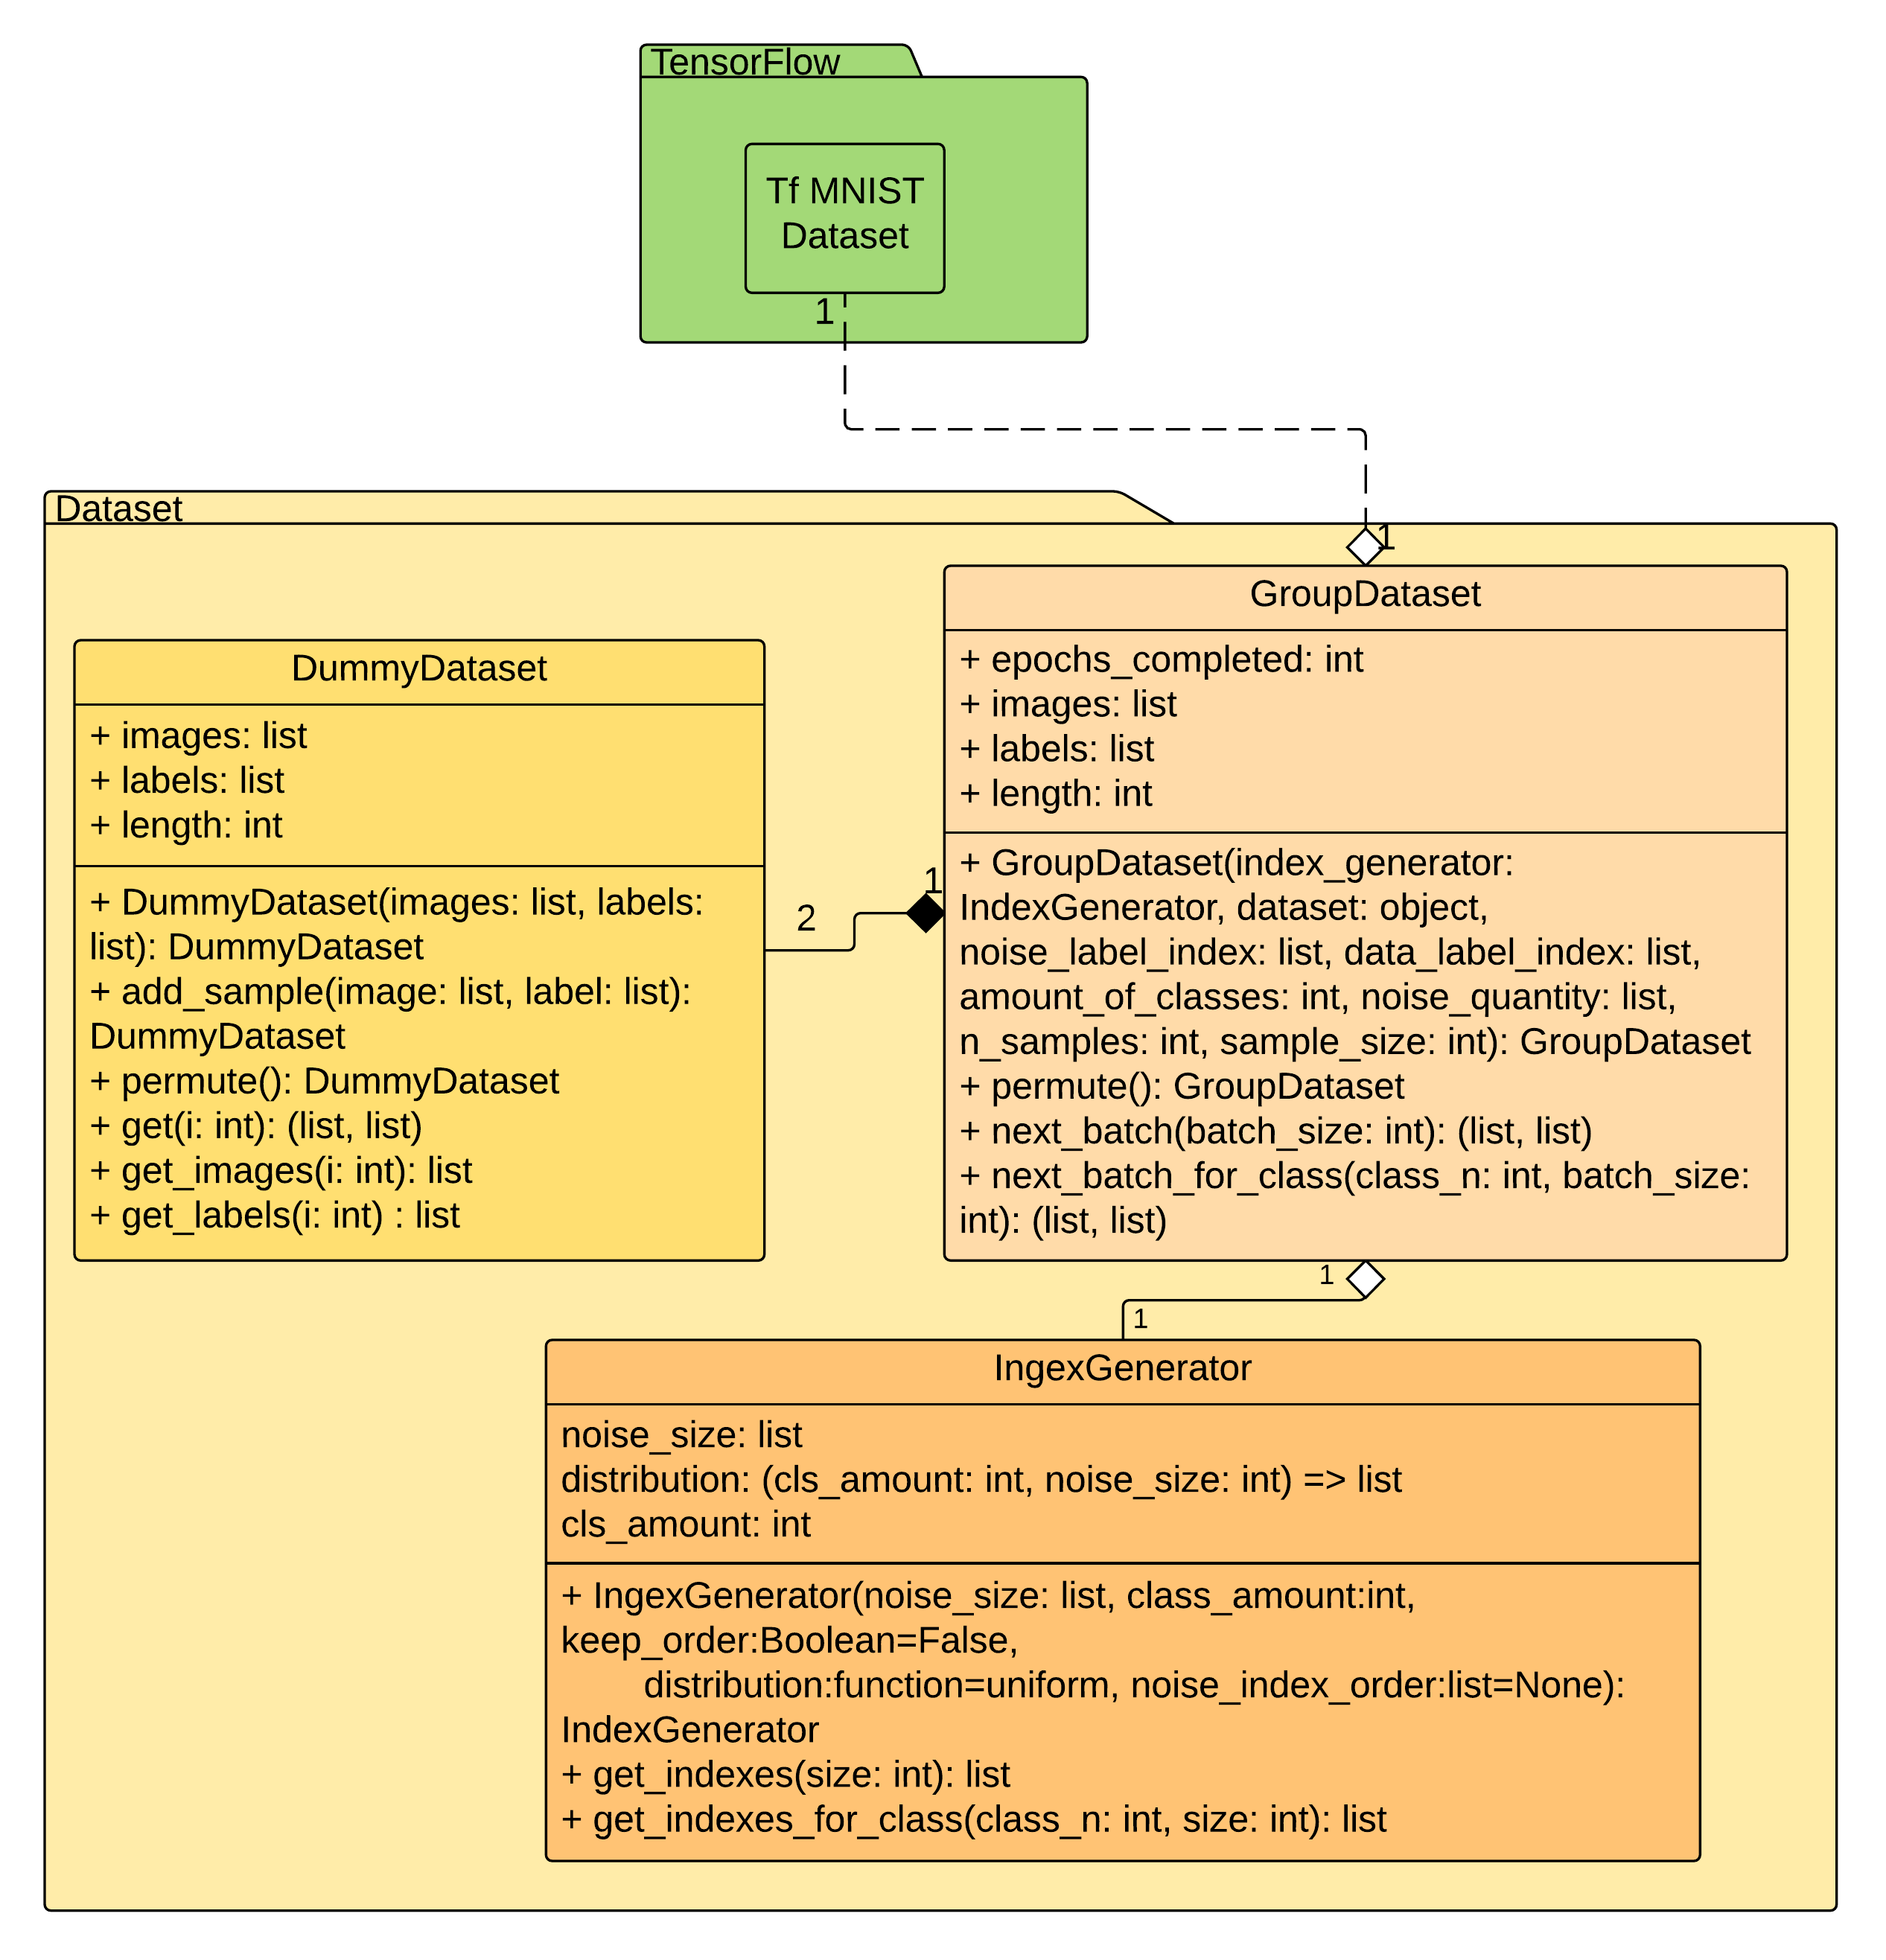
\includegraphics[width=\linewidth]{Dataset_UML}
	\caption{UML class diagram of the dataset module}
	\label{fig:dataset_uml}
\end{figure}

\paragraph{Code patterns} As we can see from the UML class in the figure
\ref{fig:dataset_uml}, we have three classes. It would be also possible
to merge the classes, however, this contradicts the "Single Responsibility Principle"
as one class should only have one responsibility \cite{martin2003agile}.
Therefore, dividing this into two classes allows us to clearly
define responsibilities. Consequently, this separation seems to be reasonable.

As you might notice from UML class diagram, some of the functions like
\lstinline{add_sample} in \lstinline{DummyDataset} returns the object itself: \lstinline{DummyDataset}.
This is an example of Cascade code pattern described in \autoref{sec:quality_concerns}.
% As you might notice from UML class diagram, that \lstinline{GroupDataset} can inherit
% \lstinline{DummyDataset} as they have similar properties,
% but as "Composition over Inhertitance" states, it
% not always a good idea.

%
% inderect variable access. (e.g.)

% TODO:
% look over the Dataset implementation,
% write all documentation
% draw uml diagrams
%
%
%
%
%

% \paragraph{Requirements} Like why do we need index generator
% including flexibility
% \paragraph{Inspiration fromt the tf class dataset}
%
% inpsiration from dataset class from tensor flow: link
% https://github.com/tensorflow/tensorflow/blob/master/tensorflow/contrib/learn/python/learn/datasets/mnist.py
% that should perform similar action to
% The function requirement to the dataset can be formulated as

% \paragraph{
% 	not learning any dependency,
% 	explain that we want to avoid the same samples in a group to avoid that
% }
% model will learn dependency and etc.

% \paragraph{
% 	explain shortly about combinations of MNIST data, how to achieve the best data
% }
%
% \paragraph{then show the uml diagram of dataset}
% including: Class overview
%
% \paragraph{explain what is purpose of each of the class. }


\section{Model}
\label{sec:design_model}

% \paragraph{Why did you choose picker network?}
We described three approaches of how to extend the RAM model
in \autoref{sec:extension}. The implementation of this work
will only concentrate on the method described as picker network.
This is because of the simplicity of this approach.

%TODO: patterns https://www.toptal.com/python/python-design-patterns

% \paragraph{about why OO programming is not ALMOST suited and why it should be more functional}
It's common practices in TensorFlow to use functions for implementing the model.
We will stick to this practice for defining the model because this can
potentially reduce the complexity of the model as well as
increase readability of the code.

% \paragraph{The architecture as a whole}

\subsection{Architecture} \label{subs:arch_model} Taking into account
the extension that was
described in \autoref{subs:picker_net}, we can easily derive classes
as each of the networks has a clear task. Building the model will be
possible using following clases:

\begin{itemize}
	\item GlimpseSensor - the class is responsible for extracting glimpses from
		images at given location $l_t$.
	\item PickerNet - this class is responsible for picking an image out of the
		group of images.
	\item GlimpseNet - given the glimpse sensor, images and number of picked image,
		this class is responsible for producing the feature map from the image,
		which is then fed into LSTM cell.
	\item LocNet - the class is responsible for producing next location for
	glimpse sensor to attend to.
	\item Model - formally, this is not a class, but a set of function that build
		and run the model. We will represent this set as a class in UML class diagram
		in \autoref{subs:uml_model}. However, this set of functions will also be explained
		more detailed in \autoref{subs:model_seq_diagramm}.
		For now, we'll refer to it as a class.
	\item Config - singleton class that holds all
		configuration parameters for the model such as shape of weights
		for hidden layers.
\end{itemize}


\subsection{UML class diagram}
\label{subs:uml_model}

In the figure \ref{fig:model_uml}, you can see the UML class diagram for the
architecture we described above. As it was already mentioned the \lstinline{Config}
class is a singleton class that holds all configuration details for the model.
Once initialised with command-line options or default values, it's a single source
of truth for the whole application. The use of singleton design pattern here helps
to avoid misconception that application can have more than one configuration.
From the UML diagram we see that only class \lstinline{Model} use the
\lstinline{Config}, this is because of the convenience sake. Without much effort the
\lstinline{Config} can be imported from other classes as well.

\begin{figure}[H]
	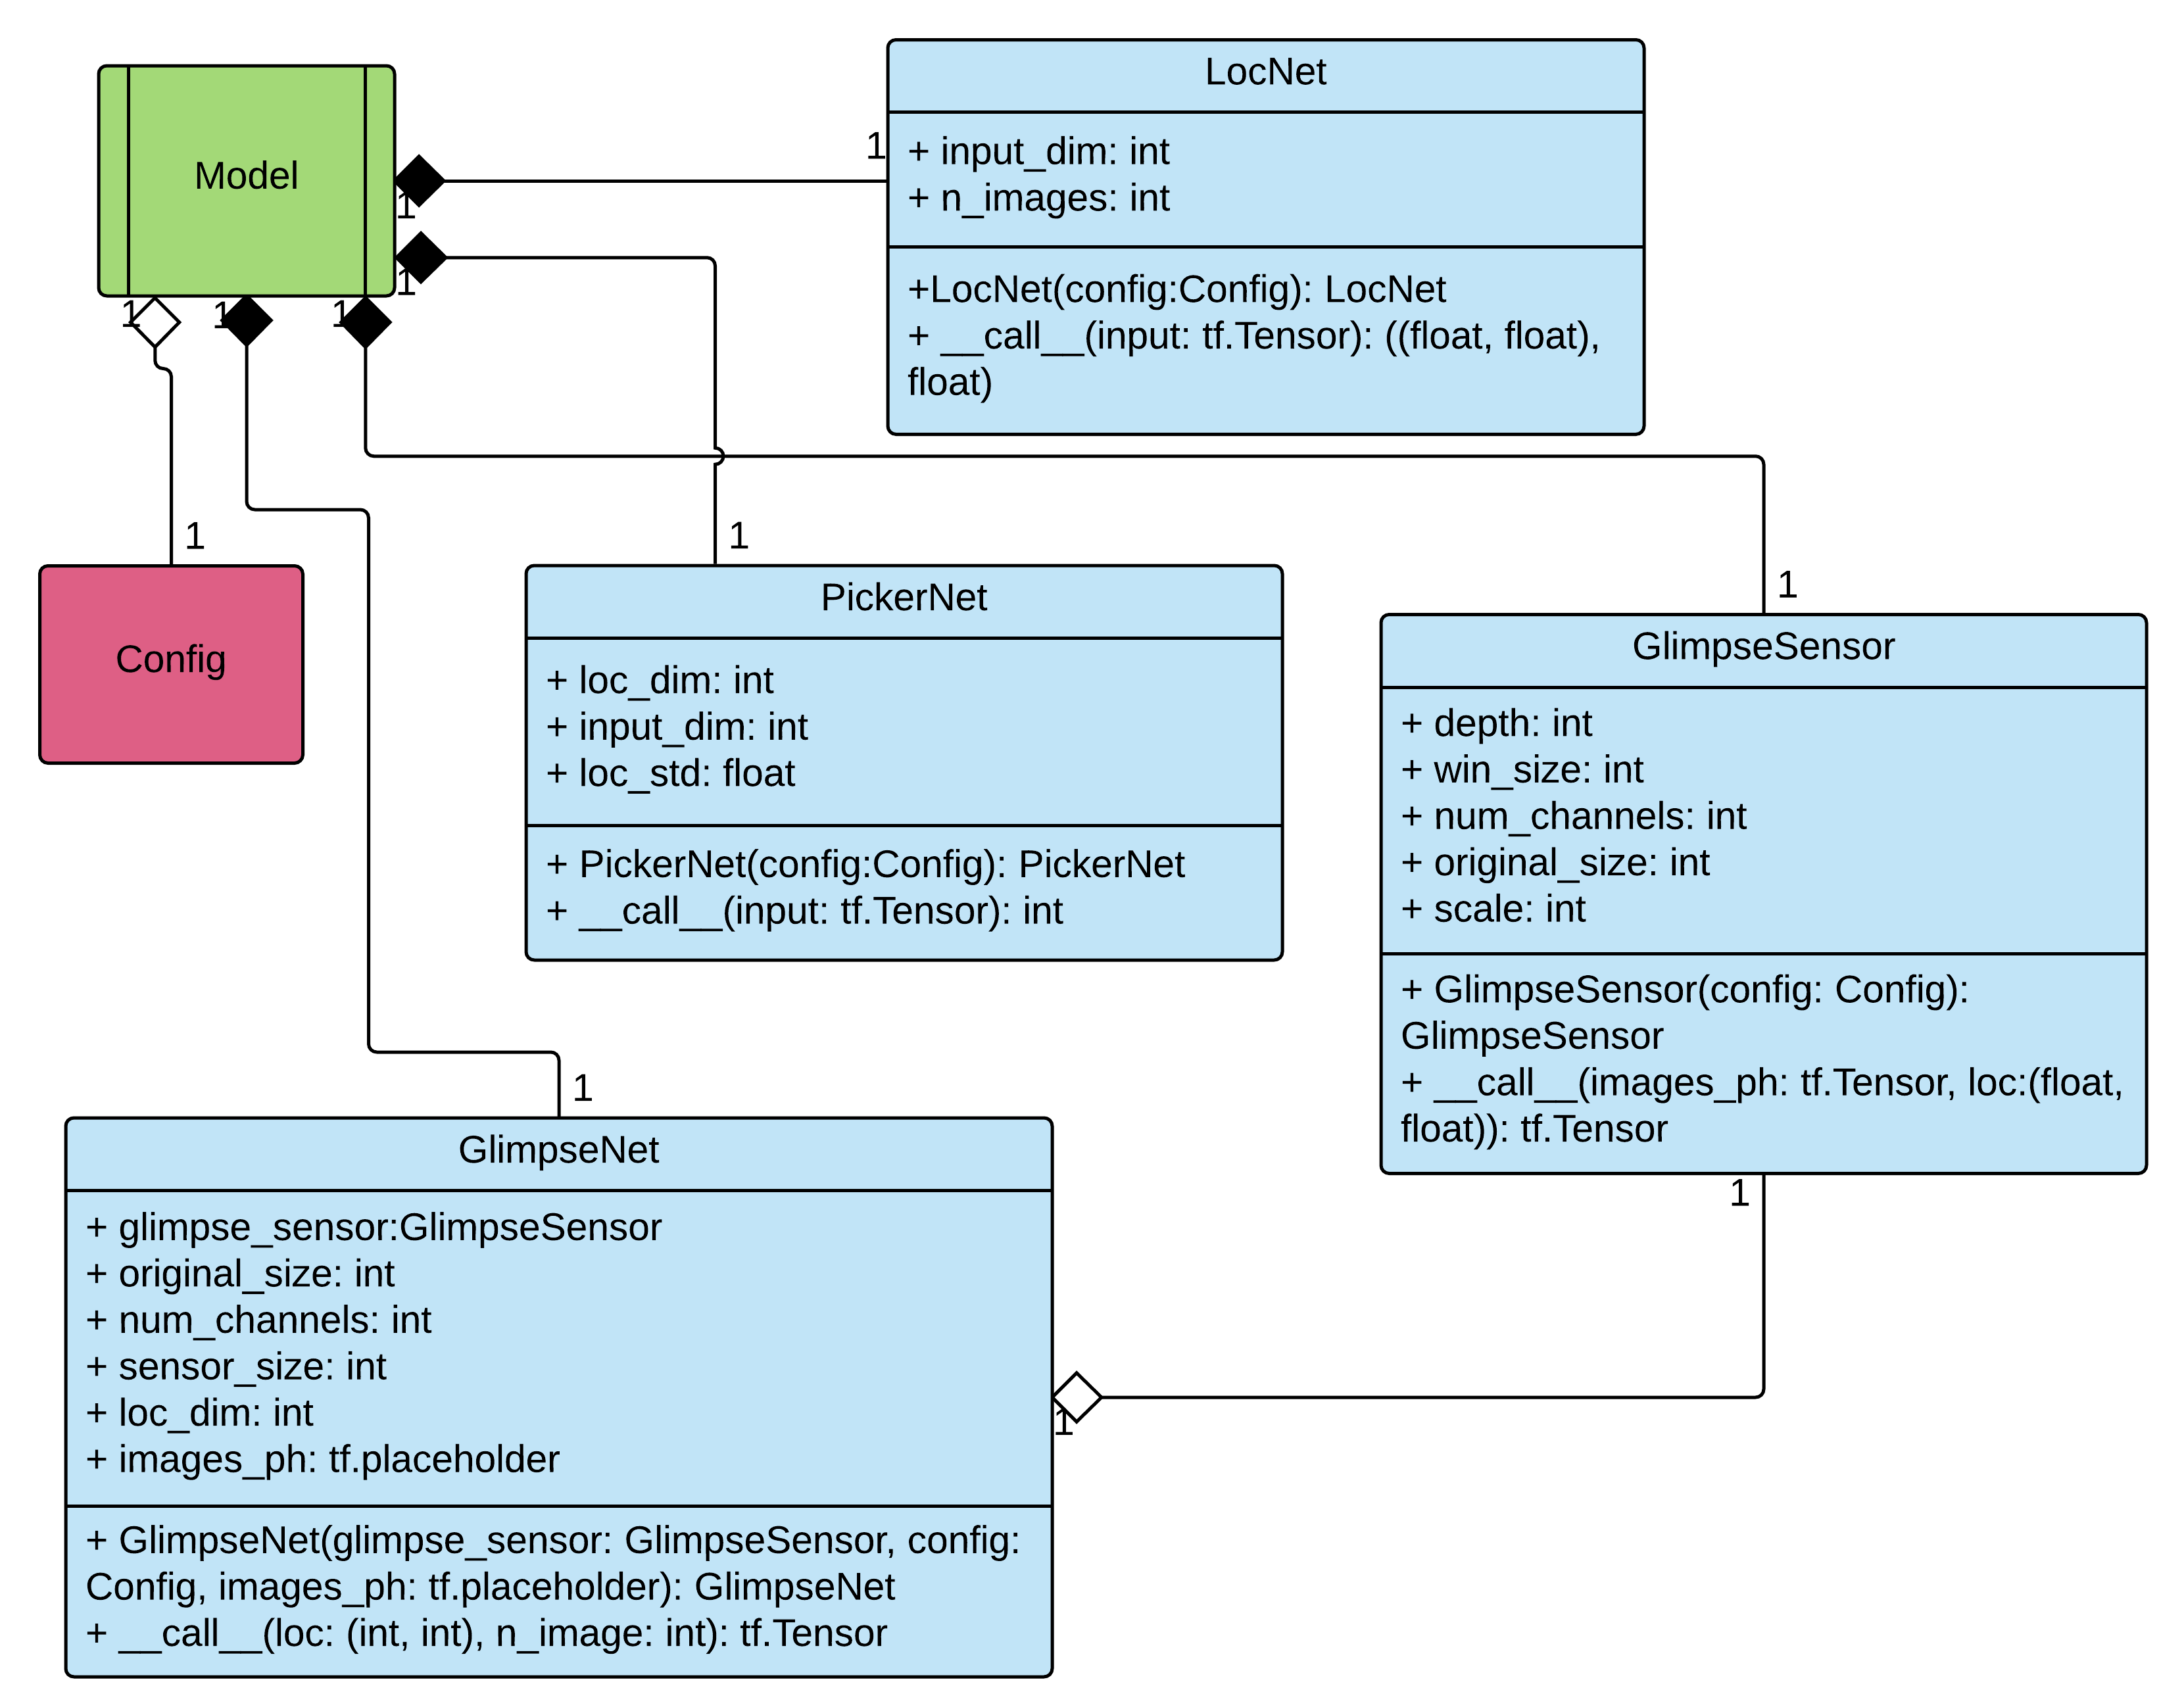
\includegraphics[width=\linewidth]{Model_UML}
	\caption{UML class diagram of the Model component}
	\label{fig:model_uml}
\end{figure}


\subsection{UML activity diagram for the Model}
\label{subs:model_seq_diagramm}
To prevent misunderstanding, we distinguish between the \lstinline{Model} class
and the Model component. Model component is a set of classes and functions related
to RAM and it's extension. The \lstinline{Model} class is a class that we described
in \autoref{subs:arch_model}.
As it was mentioned earlier, the \lstinline{Model} is not an actual class, but a set of
functions. The \lstinline{Model} class is the core of the Model component. It instantiates
other classes as well as runs, trains
and evaluates the model. Since the \lstinline{Model} contains only functions,
it's hard to represent it as UML class diagram. However, UML activity diagram
can be a good fit if we replace the activities in the UML notation with
the functions. Therefore to clarify the flow of the \lstinline{Model}, you may
find the figure \ref{fig:uml_activity_model} with the UML activity diagram helpful.
In the lane with the name \lstinline{init_seq_rnn()}, you can see a set of functions
related to LSTM cell initialisation. This lane means that inside \lstinline{init_seq_rnn()}
function this set of function is called.
The container with the name "calculate the hybrid loss", mean nothing more than
conceptual conncetion between the function inside.
We will take a closer look at some of details of this functions in the
\autoref{ch:implementation}.
% As you can see from the diagrams, the functions names can describe the
% functionality that it does. With
% \label{sec:quality_concerns}


%  To get an idea of what \lstinline{Model} does,
%
% To simplify the understanding of what the \lstinline{Model}
% consist


\begin{figure}[H]
	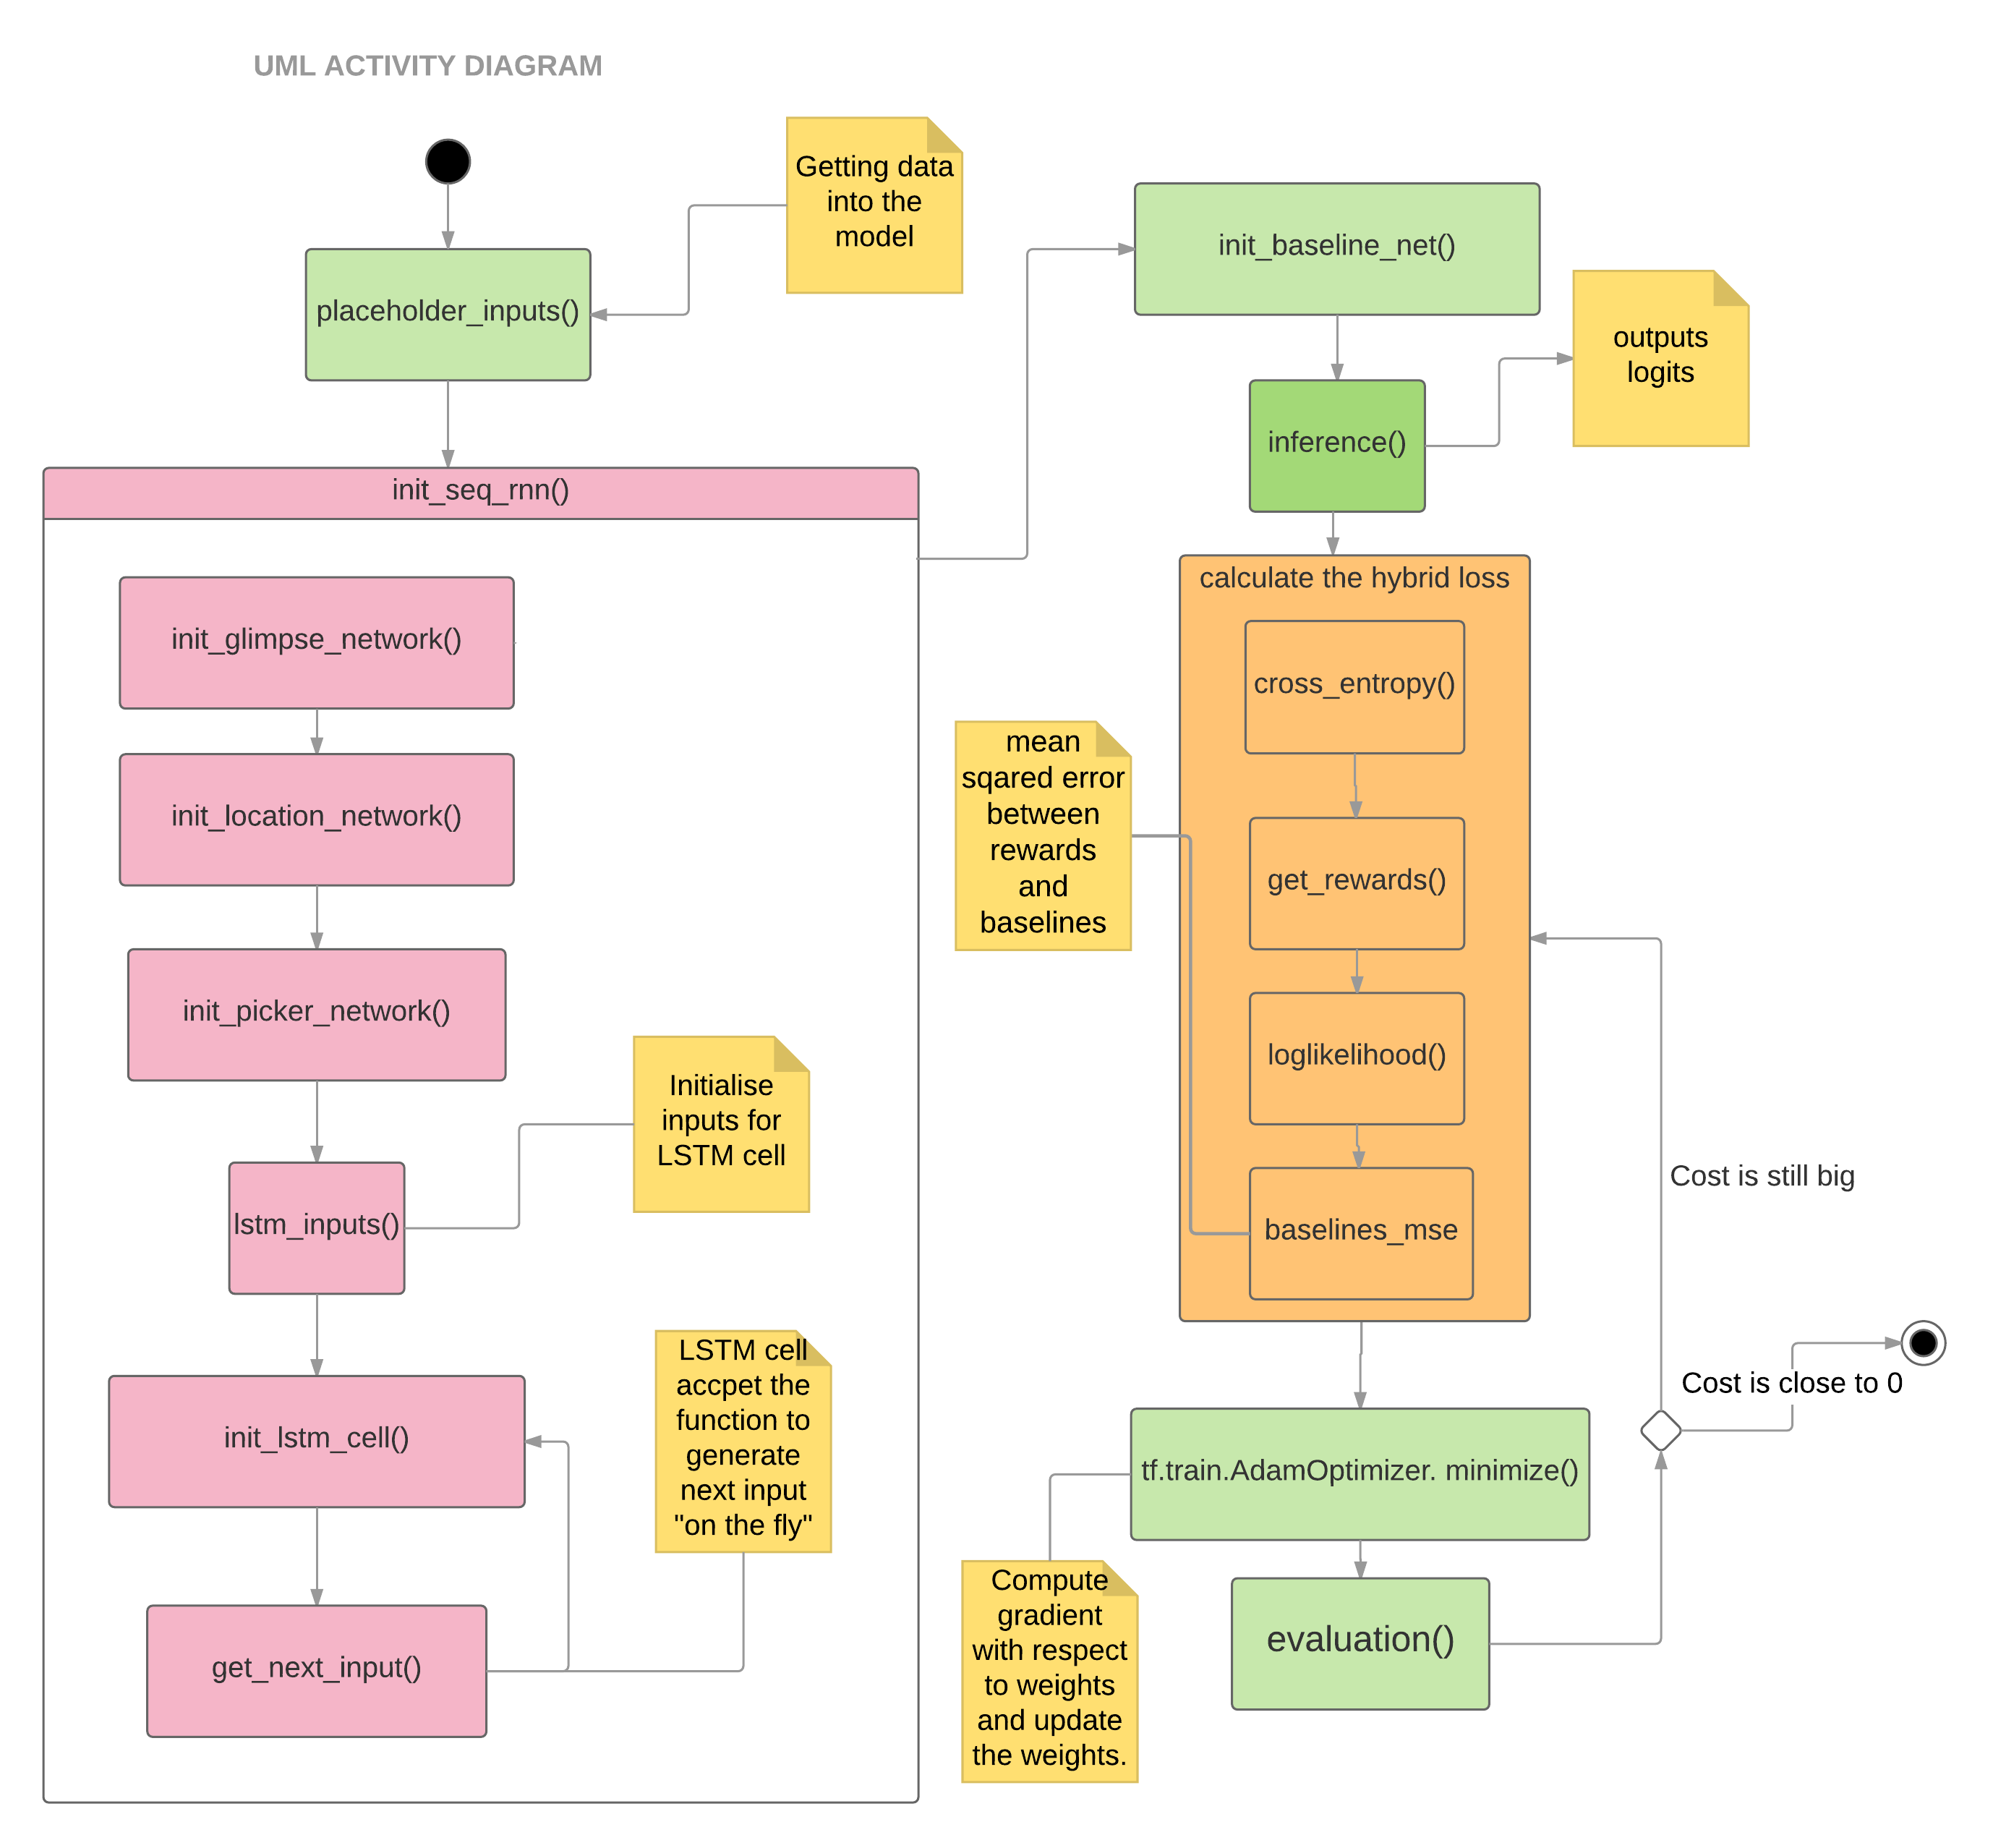
\includegraphics[width=\linewidth]{uml_activity_model}
	\caption{UML activity diagram of the Model}
	\caption*{This is simplified flow of the \lstinline{Model} class.
	Each activity represent a function. For the sake of simplicity some of the functions
	are not shown here. However, it should not influence on the understanding
	of the \lstinline{Model}}.
	\label{fig:uml_activity_model}
\end{figure}
%
% #
% Sequence:
% input(images)
% Init RNN ->
%     init_glimpse_network
%     init_location_network
%     init_picker_network
%     init lstm_inputs
%     init LSTM cell
%     defined the next input function for LSTM (get_next_input) --> depends on the all above
%     -> outputs
% init_baseline_net(outputs)
% cross_entropy(logits, groud_truth)
% get_rewards(pred_labels, labels_ph) --> calculate rewards
% define loglikelyhood ratio
% defined hybrid loss
% train the model with AdamOptimizer with respect to loss.
% #
% the plan:
% draw uml diagram: represent the main run_training as a class.
% make a note that it's actually not a class but a set of functions to
% to represent the model.
% then draw this main class again with the explanation of how the
% things is working using any sequential type of diagram.
% Config is singleton
% \paragraph{Possible classes, overview}
% \paragraph{UML diagram}
% \paragraph{back up the classes with design patterns}
%
% \paragraph{the flow of the data via function}


% \subsection{Configuration of the project, what can be configured, the complexity of the model}




% write about configuration file in implementation
% the curent desing is using the approach
% described in \autoref{ssec:picker_net}.
%
% Basically explain the flow of input data, all losses, and baselines, and etc.
% if there is anything relative to the structure in the code use the references to the design patters
% Show all classes, write the documentation for those, or at least briefly explain the purpose.
% The process of training, maybe explain the whole idea behind this
% 	seperation of dataset into validation, test, training.
% look at the other bachelorarbeits and look of what they wrote there
% think about whether it's possible to combine the design and implemntation chapters
%
%
%
% * Entwurfsstrategie, Beschreibungen funktionaler und nich
%  funktionaler Anforderungen, Einsatz von Mustern und
%  Bibliotheken, Softwarearchitektur, Verwendung von Datentypen und
%  Datenstrukturen, Algorithmen, Mensch-Maschine-Schnittstelle;
